\documentclass[tikz,border=5pt]{standalone}
% -- -- -- -- -- -- -- -- -- -- -- -- -- -- -- -- -- -- -- -- -- -- -- -- -- --
\begin{document}
% -- -- -- -- -- -- -- -- -- -- -- -- -- -- -- -- -- -- -- -- -- -- -- -- -- --
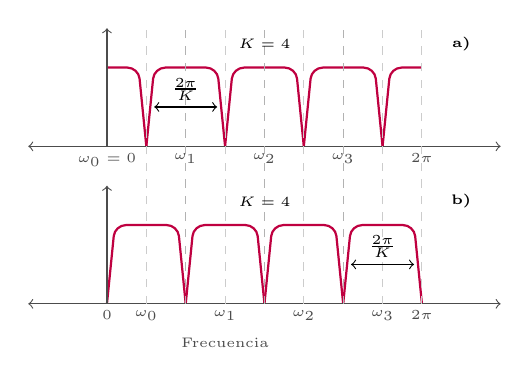
\begin{tikzpicture}
				%\draw[step=0.5,help lines] (-2,-1) grid (8,4);
\tiny
% body of the graph
				\foreach \i in {0,1,2,3}
				\draw [purple, thick, rounded corners] (\i,0) -- (\i+0.1,1) -- (\i+0.9,1) --	(\i+1,0);
				\foreach \i in {0,1,2}
				\draw [purple, thick, rounded corners] (\i+0.5,2) -- (\i+0.1+0.5,3) --
				(\i+0.9+0.5,3) --	(\i+1+0.5,2);
				\draw [purple, thick, rounded corners] (0,3) -- (0.5-0.1,3) -- (0.5,2);
				\draw [purple, thick, rounded corners] (3.5,2) -- (3.5+0.1,3) -- (4,3);
			%	\foreach \i in {1,2,3,4}
			%	\draw [purple, thick, rounded corners] (\i+0.1,4) -- (\i+0.2+0.1,5) --
			%	(\i+0.8-0.1,5) --	(\i+1-0.1,4);
% draw axis
    %\draw[->,black!70] (0,4) -- (0,5.5); 
    \draw[->,black!70] (0,2) -- (0,3.5); %\draw(-0.3,2.7) node[rotate=90]	{Amplitud};
    \draw[->,black!70] (0,0) -- (0,1.5);
    \draw[<->,black!70] (-1,0) -- (5,0);% node[below] {$\omega'$};
    \draw[<->,black!70] (-1,2) -- (5,2);% node[below] {$\omega'$};
    %\draw[->,black!70] (0,4) -- (6,4);% node[below] {$\omega'$};
% draw axis label
    \draw[black!70] (0.0,0) node[below] {$0$};
    \draw[black!70] (4.0,2) node[below] {$2\pi$};
    \draw[black!70] (4.0,0) node[below] {$2\pi$};
				\draw[black!70] (1.5,-0.5) node[] {Frecuencia};
				\draw[black!70] (0,2) node[below] {$\omega_0=0$};
				\draw[black!70] (1,2) node[below] {$\omega_1$};
				\draw[black!70] (2,2) node[below] {$\omega_2$};
				\draw[black!70] (3,2) node[below] {$\omega_3$};

				\draw[black!70] (0.5,0) node[below] {$\omega_0$};
				\draw[black!70] (1.5,0) node[below] {$\omega_1$};
				\draw[black!70] (2.5,0) node[below] {$\omega_2$};
				\draw[black!70] (3.5,0) node[below] {$\omega_3$};

				\draw [black!20, dashed] (0.5,0) -- (0.5,3.5);
				\draw [black!20, dashed] (1.5,0) -- (1.5,3.5);
				\draw [black!20, dashed] (2.5,0) -- (2.5,3.5);
				\draw [black!20, dashed] (3.5,0) -- (3.5,3.5);
				\draw [black!20, dashed] (4,0) -- (4,3.5);

				%\draw [black!30, dashed] (0.0,0) -- (0.0,3.5);
				\draw [black!30, dashed] (1.0,0) -- (1.0,3.5);
				\draw [black!30, dashed] (2.0,0) -- (2.0,3.5);
				\draw [black!30, dashed] (3.0,0) -- (3.0,3.5);

				%\draw [black!20, dashed] (4.5,0) -- (4.5,5.5);
				\draw[<->] (0.6,2.5) -- (1.4,2.5) node[above,scale=1,xshift=-0.4cm] {$\frac{2\pi}{K}$};
				\draw[<->] (3.1,0.5) -- (3.9,0.5) node[above,scale=1,xshift=-0.4cm] {$\frac{2\pi}{K}$};

				\node at (2,3.3) {\textbf{$K=4$}};
				\node at (2,1.3) {\textbf{$K=4$}};
				\node at (4.5,3.3) {\textbf{a)}};
				\node at (4.5,1.3) {\textbf{b)}};

\end{tikzpicture}
% -- -- -- -- -- -- -- -- -- -- -- -- -- -- -- -- -- -- -- -- -- -- -- -- -- --
\end{document}
